\documentclass[10pt, a4paper]{beamer}

\usetheme{Berkeley}
\usecolortheme{sidebartab}

\begin{document}
	\setbeamertemplate{sidebar left}{}
	\title{Progress Presentation-I}
	\subtitle{e-Yantra Summer Internship-2015 \\ PC CONTROLLED TWO WHEEL BALANCE BOT}
	\author{B Suresh\\Ramiz Hussain\\Devendra Kumar Jangir \\
	Mentors: Piyush Manavar,Saurav Shandilya}
	\institute{\textbf{IIT Bombay}}
	\date{\today}
	%\addtobeamertemplate{sidebar left}{}{\includegraphics[scale = 0.3]{logowithtext.png}}
	\frame{\titlepage}

\setbeamertemplate{sidebar left}[sidebar theme]
\section{Overview of Project}
\begin{frame}{Overview of Project}
	%$Give following details: \\
	\begin{itemize}
		\item \textbf{Project Name} :PC controlled two wheel balanced bot
		\item \textbf{Objective} : To make a two wheel balance bot which can balance itself without any extra support.
		\item \textbf{Deliverables}: \\
		\begin{enumerate}
			\item Two wheel balance bot
			\item PC controlled motion
			\item Documentation and tutorials
			\item Sample code
		\end{enumerate}
		\end{itemize}
\end{frame}

\section{Image}
\begin{frame}{Image}
	\begin{figure}
	  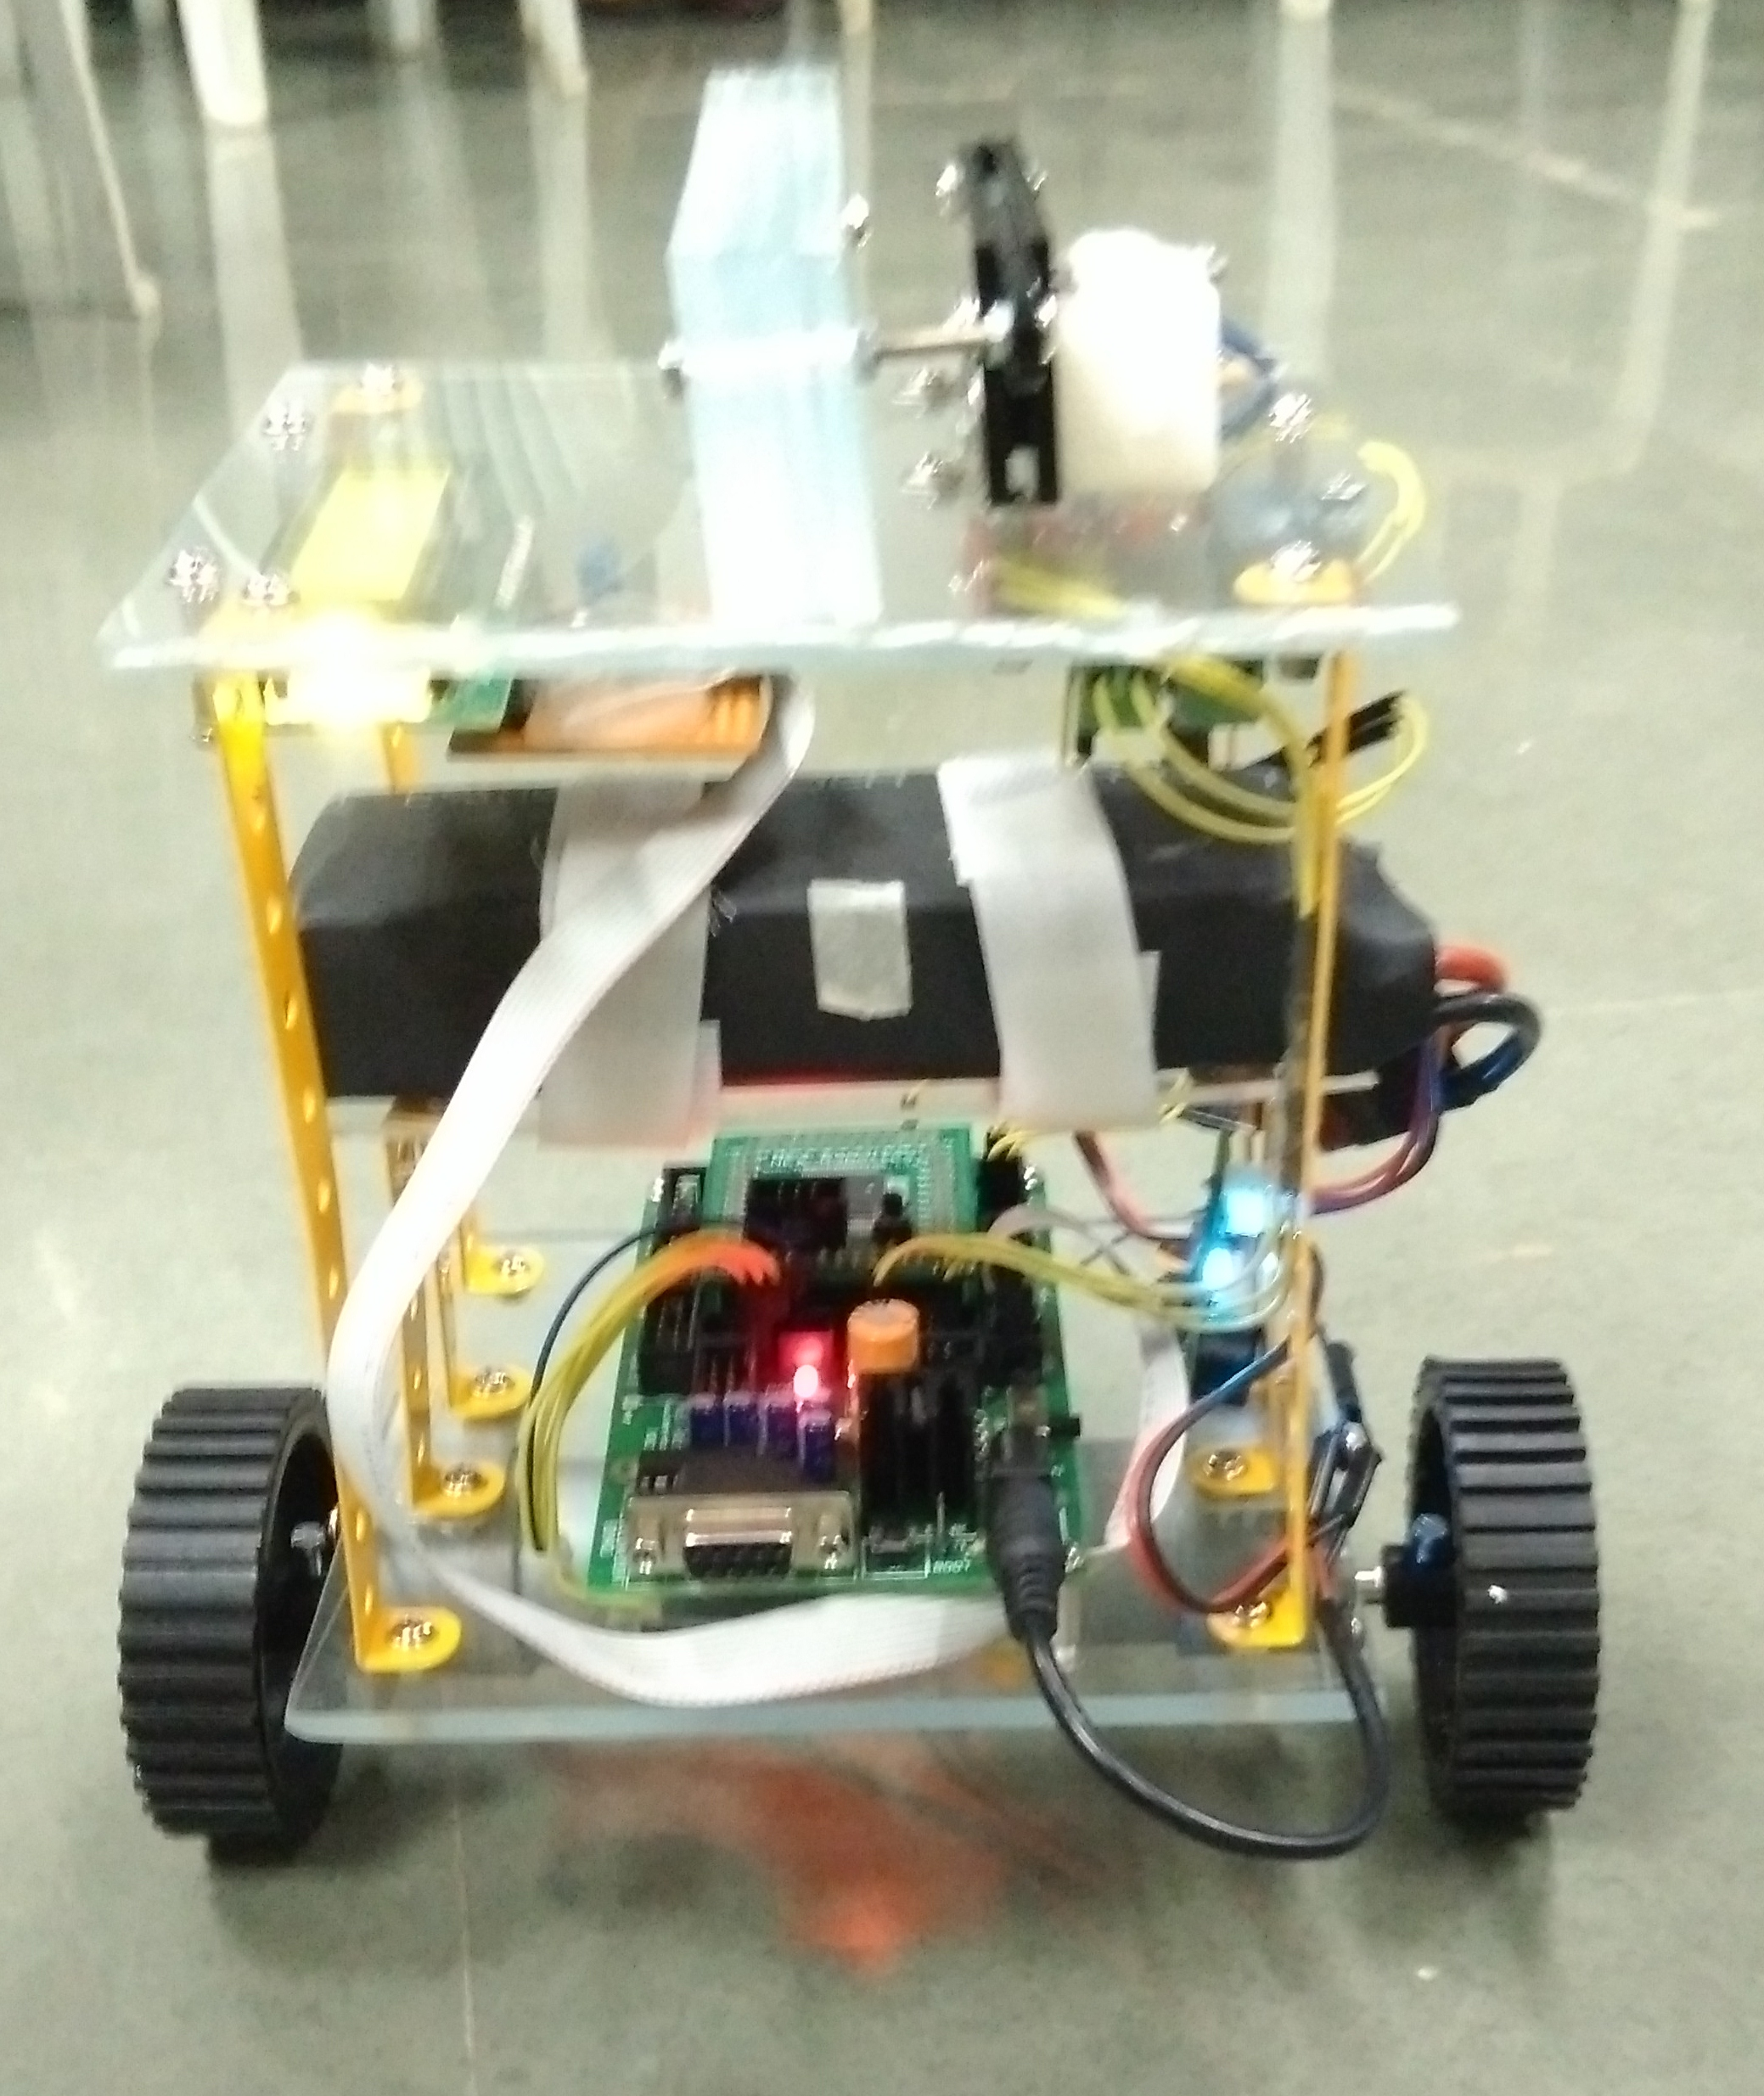
\includegraphics[scale=0.1]{Balance_bot.jpg}
	\end{figure}
\end{frame}

\section{Overview of Task}
\begin{frame}{Overview of Task}
	\small
        \begin{tabular}{|c|p{6cm}|c|}
        \hline
         \textbf{Task No.} & \centering {\textbf{Task}} & \textbf{Deadline} \\ 
         \hline
		1 & Selection of components, sensors \quad and \quad actuators & week 1\\
		\hline 
		2 & Design and fabrication of bot & week 1 \\
		\hline 
		3 & Designing of circuit,power management and interfacing & week 1 \\
		\hline
		4 & Algorithm and code implementation for \quad balancing & week 2,3 \\
		\hline
		5 &  Algorithm and code implementation for \qquad  locomotion via PC communication & week 4,5 \\
		\hline 
		6 & Analysis and documentation & week 6 \\
		\hline 
        \end{tabular}
\end{frame}

\section{Task Accomplised}
\begin{frame}{Task Accomplised}
	\textbf{TASK1:Selection of components,sensors and actuators} 
    \begin{enumerate}
     \item ATmega 2560 Development board
     \item DC Motor(300 RPM)
     \item Linear Actuator(150 RPM)
     \item L293D and L298N Motor driver
     \item 16x2 LCD Display
     \item GY-80(Accelerometer and Gyroscope module)
     \item 3 cell Li Po battery 11.1 Volts
     \item Xbee module and adapter
    \end{enumerate}
\end{frame}

\section{Task Accomplished}
\begin{frame}{Task Accomplished}
	\textbf{TASK2:Design and fabrication of bot}
	\begin{enumerate}
		\item Fabricating materials
		\item Weight Shifting mechanism
		\item Center of gravity
		\item Protection from falling  
	\end{enumerate}
\end{frame}


\section{Task Accomplished}
\begin{frame}{Task Accomplished}
	\textbf{TASK3:Circuit design,power management and interfacing}
	\begin{enumerate}
		\item L293D and L298N Interfacing
		\item LCD(16x2) 
		\item GY-80(ADXL345 and AGD8) Interfacing 
		\item Protection circuit for battery 
	\end{enumerate}
\end{frame}


\section{L293D Interfacing}
\begin{frame}{L293D Interfacing}
	\begin{figure}
		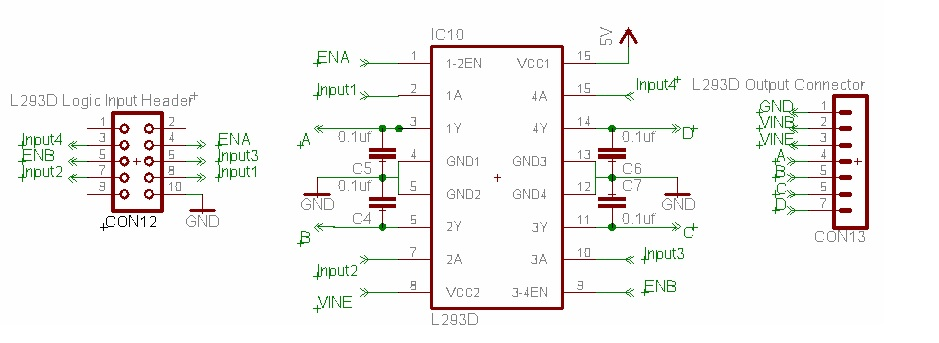
\includegraphics[scale=0.4]{L293d.jpg}
	\end{figure}
\end{frame}

\section{L298N Interfacing}
\begin{frame}{L298N Interfacing}
	\begin{figure}
		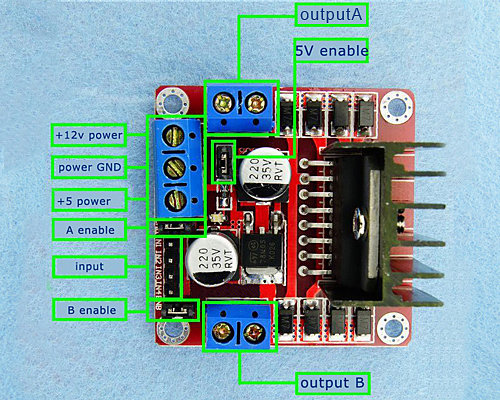
\includegraphics[scale=0.03]{l298n.jpg}
	\end{figure}
\end{frame}

\section{LCD Interfacing}
\begin{frame}{LCD Interfacing}
	\begin{figure}
		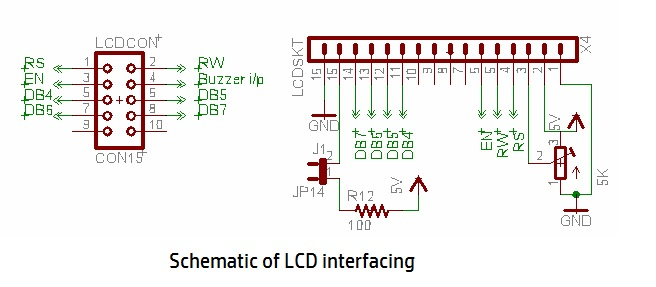
\includegraphics[scale=0.5]{LCD.jpg}
	\end{figure}
\end{frame}

\section{GY-80 Module Interfacing}
\begin{frame}{GY-80 Module Interfacing}
	\begin{figure}
		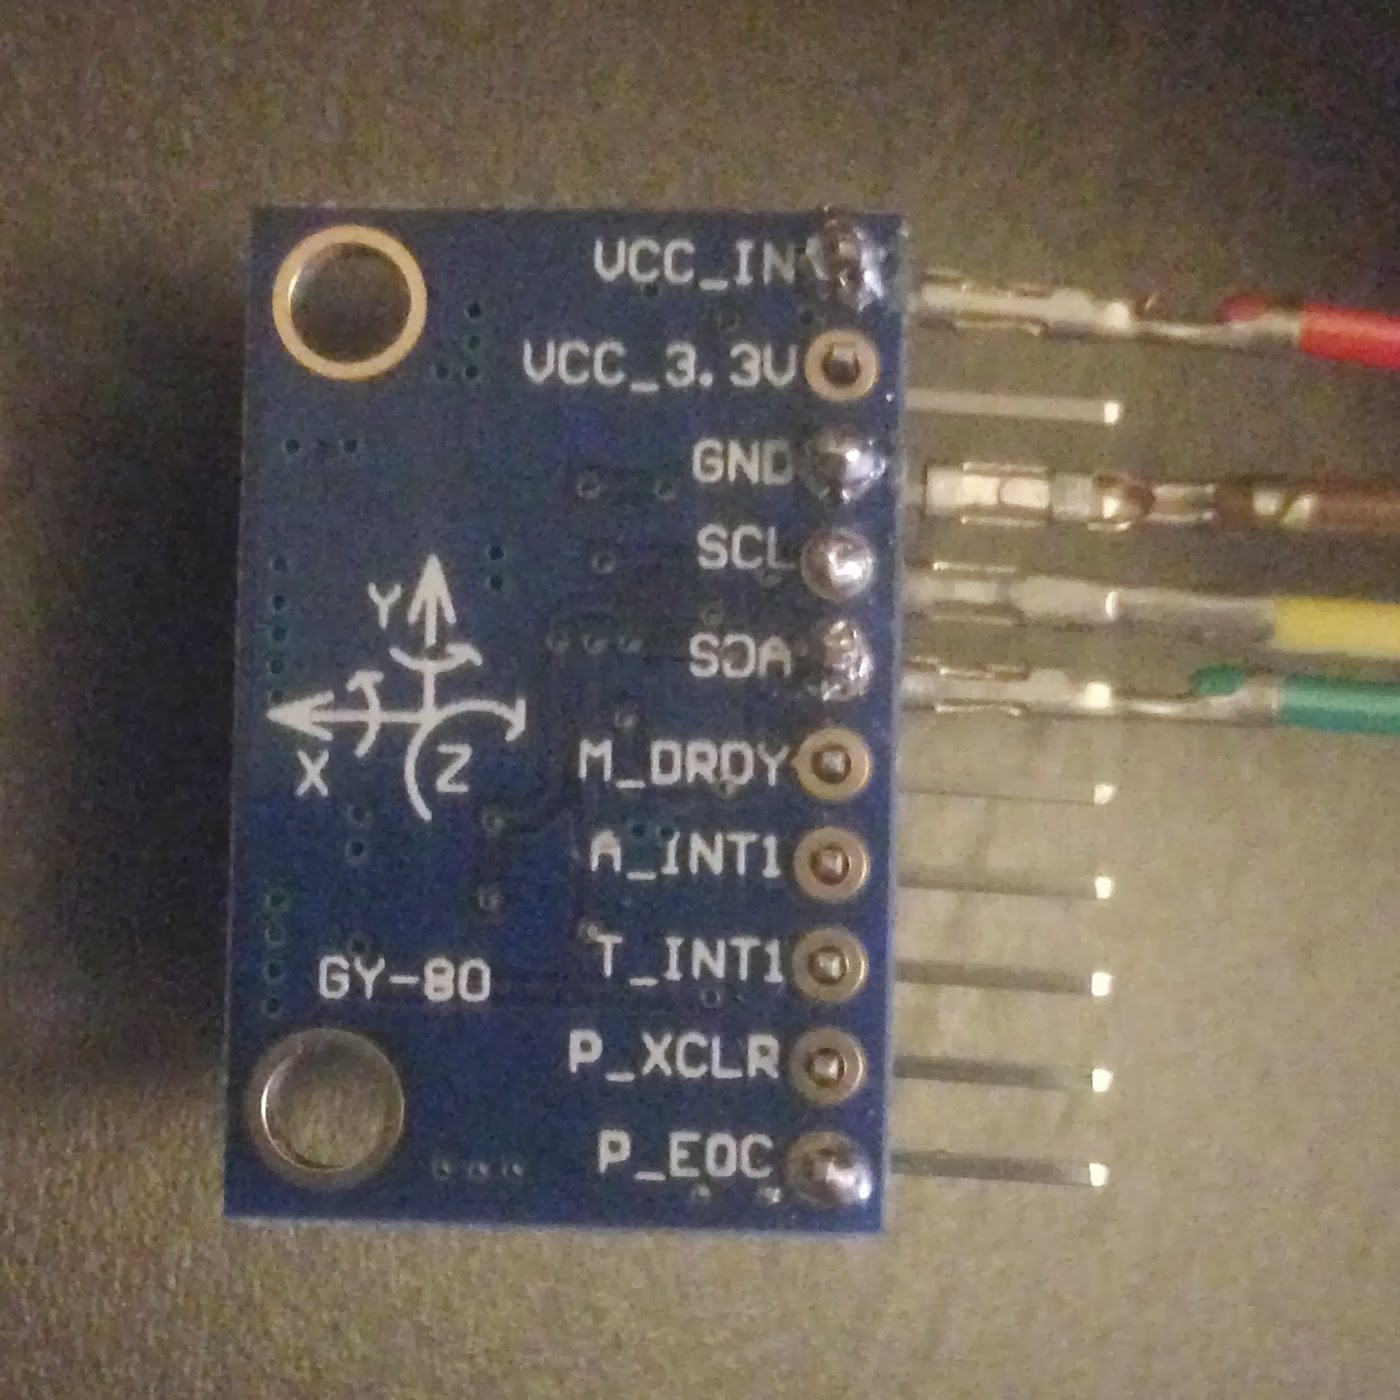
\includegraphics[scale=0.15]{gy80.jpg}
	\end{figure}
\end{frame}



\section{Task Accomplished}
\begin{frame}{Task Accomplished}
	\textbf{TASK4:Algorithm and code implementation}
	\begin{enumerate}
		\item I2C protocol for accelerometer and gyroscope
		\item PWM(10bit Fast PWM or Phase Correct PWM) for controlling velocity of motors 
		\item Timers for PWM and PID calculations
		\item PID Algorithm for balancing the bot 
	\end{enumerate}
\end{frame}


\section{I2C protocol}
\begin{frame}{I2C Protocol}
	\begin{itemize}
		\item It is a synchronous data transfer protocol and uses master/slave technique.
		\item Maste initiates the communication .
		\item Slave works according to the master.
		\item Multiple devices can connect at the same time,each having a unique 7-bit address.
		\item Two bidirectional lines used for communication are:SCL(Serial clock) and SDA(Serial Data) 
	\end{itemize}
\end{frame}


\section{I2C software protocol}
\begin{frame}{I2C software protocol}
	\begin{figure}
		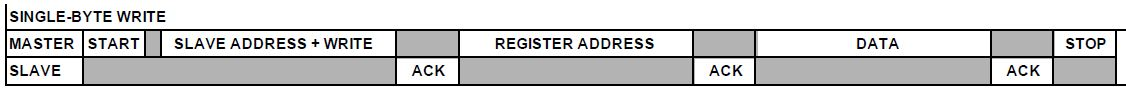
\includegraphics[scale=0.35]{I2C_write.jpg}\\
		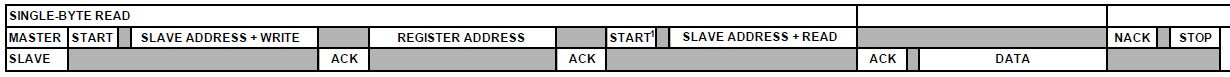
\includegraphics[scale=0.33]{I2C_read.jpg}
	\end{figure}
\end{frame}

\section{PID algorithm for the bot}
\begin{frame}{PID algorithm for the bot}
	\begin{figure}
		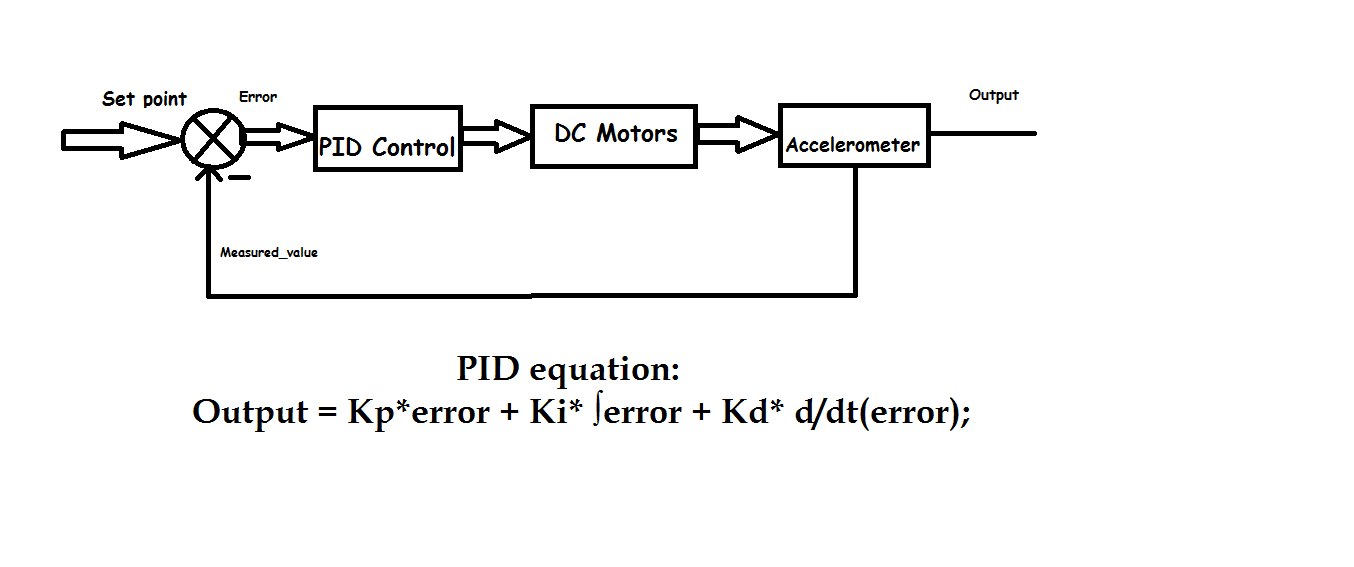
\includegraphics[scale=0.35]{PID.png}\\
		
	\end{figure}
\end{frame}

\section{Challenges faced}
\begin{frame}{Challenges Faced}
	\begin{itemize}
	 \item Maintaining Center Of Gravity(COG) while fabricating the bot
	 \item Understanding and Implementing I2C protocol
	 \item Converting accelerometer values to angles in degrees
	 \item Erroneous reading from accelerometer
	 \item Generating time function using 16 bit timer
	 \item PID tuning  
	 \end{itemize}
\end{frame}

\section{Future Plans}
\begin{frame}{Future Plans}
	\begin{itemize}
		\item PID implementation for balancing and moving the bot
		\item Integrating gyroscope values using Complementary filter
		\item Xbee interfacing 
	\end{itemize}
\end{frame}


\section{Thank You}
\begin{frame}{Thank You}
	\centering THANK YOU !!!
\end{frame}
\end{document}
